\documentclass[tikz, preview=true, border=2mm]{standalone}

\usepackage{xcolor}
\colorlet{myred}{red!80!black}
\colorlet{myblue}{blue!80!black}
\colorlet{mybluee}{myblue!80!black}
\colorlet{mygreen}{green!50!black}
\colorlet{myorange}{orange!70!red!60!black}
\colorlet{mydarkred}{red!30!black}
\colorlet{mydarkblue}{blue!40!black}
\colorlet{mydarkgreen}{green!30!black}

\renewcommand*\familydefault{\sfdefault}

\usepackage{tikz}
\usetikzlibrary{mindmap,trees,shadows}

\begin{document}

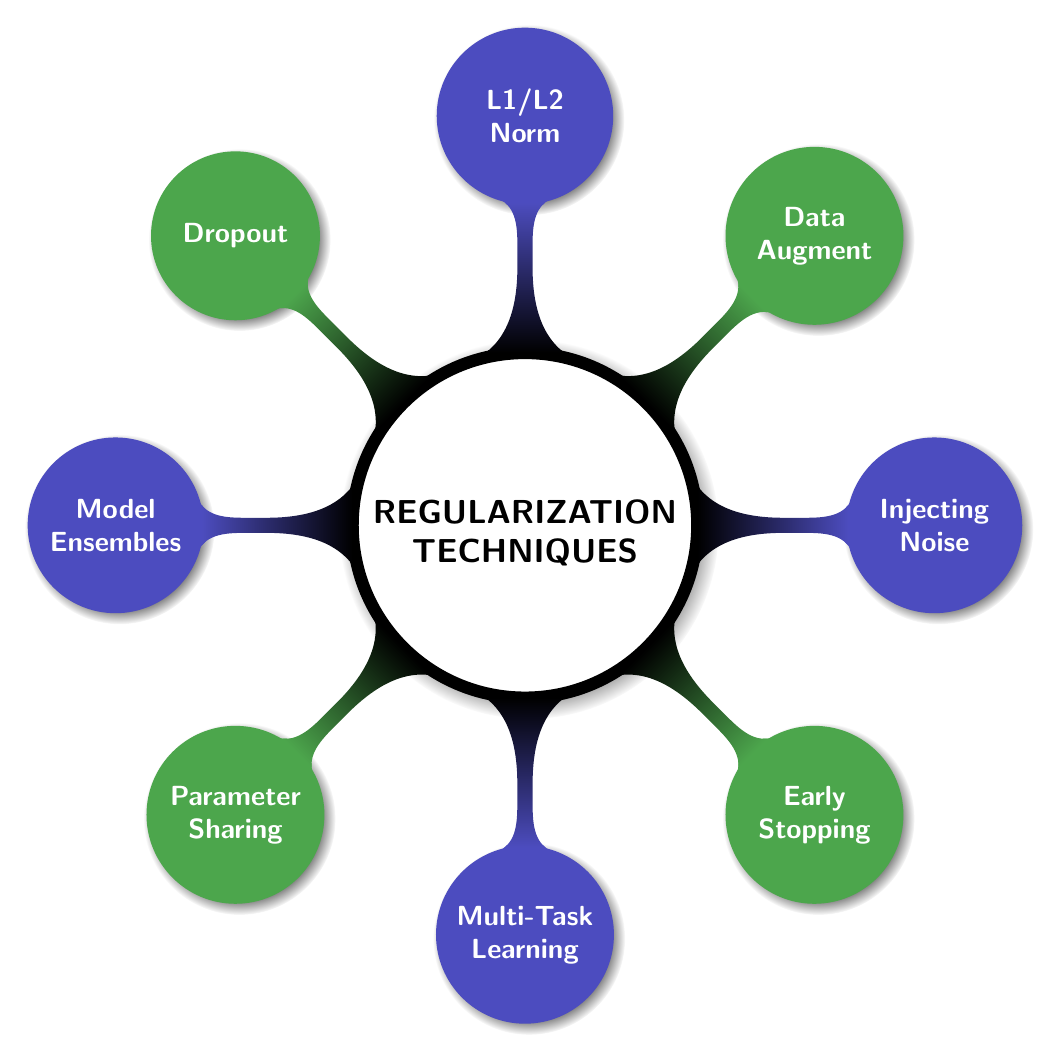
\begin{tikzpicture}
    [decoration={start radius=1cm, end radius=.5cm,amplitude=3mm,angle=30}]

    \begin{scope}[mindmap,
        every node/.style={concept, circular drop shadow, minimum size=0pt,execute at begin node=\hskip0pt, font=\bfseries},
        root concept/.append style={
        concept color=black, fill=white, line width=1ex, text=black, text width={width("REGULARIZATIONNNNNN")}, font=\large\scshape\bfseries,},
        level 1 concept/.append style={font=\bfseries},
        text=white,
        partner/.style={},
        grow cyclic,
        level 1/.append style={level distance=5.2cm,sibling angle=45}]
        
        \node [root concept] (team) {\ \\ REGULARIZATION\\TECHNIQUES}[rotate=202.5] % root
        child [partner, style={concept color=mygreen!70!white}] { node {Data Augment}
        }
        child [partner, style={concept color=mybluee!70!white}] { node {L1/L2 Norm}
        }
        child [partner, style={concept color=mygreen!70!white}] { node {Dropout}
        }
        child [partner, style={concept color=mybluee!70!white}] { node {Model Ensembles}
        }
        child [partner, style={concept color=mygreen!70!white}] { node {Parameter Sharing}
        }
        child [partner, style={concept color=mybluee!70!white}] { node {Multi-Task Learning}
        }
        child [partner, style={concept color=mygreen!70!white}] { node {Early Stopping}
        }
        child [partner, style={concept color=mybluee!70!white}] { node {Injecting Noise}
        };
    \end{scope}

    % \begin{scope}[xshift=4.5cm, yshift=-6cm,every node/.style={align=left,text=black}]
    %     \matrix[row sep=0pt,column sep=1mm, align=left, nodes={align=left, anchor=east}] {
    %     \node{Against of}; & \fill [mybluee!80] (0,.25ex) circle (1ex);\\
    %     \node{In Favour of}; & \fill [mygreen] (0,.25ex) circle (1ex); \\
    %     };
    % \end{scope}
\end{tikzpicture}

\end{document}